\documentclass[11pt,a4paper]{report}

\usepackage[utf8]{inputenc}
\usepackage[T1]{fontenc}
\usepackage[top=2cm,bottom=2cm,left=2.5cm,right=2.5cm]{geometry}
\usepackage{amsmath,amsfonts,amssymb}
\usepackage{graphicx}
\usepackage{subcaption}
\usepackage{inconsolata}
\usepackage{array}
\usepackage{color}
\usepackage{tcolorbox}
\usepackage{fancyhdr}
\usepackage[export]{adjustbox}
\usepackage[french]{babel}
\usepackage{listings}
\usepackage{hyperref}
\usepackage{transparent}
\usepackage{eso-pic}
\usepackage{chngpage}
\usepackage{shorttoc}
\usepackage{comment}
\usepackage{makeidx}
\usepackage[backend=biber]{biblatex}
\addbibresource{bibliographie/biblio.bib}
\usepackage{csquotes}
\usepackage{multirow}
\usepackage{footnotehyper}
\usepackage{xcolor}

\lstset{ 
    language=Python,                     % Langage
    basicstyle=\ttfamily\footnotesize,   % Style de base
    keywordstyle=\color{blue},           % Style des mots-clés
    commentstyle=\color{green},          % Style des commentaires
    stringstyle=\color{red},             % Style des chaînes de caractères
    numbers=left,                        % Numérotation des lignes
    numberstyle=\tiny\color{gray},       % Style des numéros de ligne
    stepnumber=1,                        % Numérotation chaque ligne
    numbersep=5pt,                       % Distance entre les numéros de ligne et le code
    showspaces=false,                    % Ne pas afficher les espaces
    showstringspaces=false,              % Ne pas afficher les espaces dans les chaînes de caractères
    tabsize=4,                           % Taille des tabulations
    captionpos=b,                        % Position des légendes (en bas)
    breaklines=true,                     % Retour à la ligne automatique
    breakatwhitespace=false,             % Retour à la ligne uniquement dans les espaces
    frame=single,                        % Cadre autour du code
    framerule=0.5pt,
    rulecolor=\color{black},
}


\pagestyle{fancy}

\setlength{\headheight}{25.22153pt}
\setlength{\footskip}{37.6175pt}

\definecolor{backcolour}{rgb}{0.96,0.96,0.95}
\definecolor{lightbrown}{rgb}{0.71, 0.40, 0.11}
\definecolor{myblue}{rgb}{0.3,0.4,0.9}
\definecolor{green}{rgb}{0.0, 0.5, 0.0}
\definecolor{aurometalsaurus}{rgb}{0.43, 0.5, 0.5}
\definecolor{babyblue}{rgb}{0.54, 0.81, 0.94}
\definecolor{bronze}{rgb}{0.8, 0.5, 0.2}
\definecolor{brilliantrose}{rgb}{1.0, 0.33, 0.64}

\newcommand{\dps}{\displaystyle}

\fancypagestyle{plain}{
  \fancyhead[L]{Livrable Stage M1 \\ Clément THIBAULT}
  \fancyhead[R]{\includegraphics*[width=0.2\textwidth]{images/newCerfacs+Fond.png}}
  \fancyfoot[C]{page \thepage}
  \fancyfoot[R]{\includegraphics*[width=0.1\textwidth]{images/ipsagarde.png}}
}

\fancyhead[L]{Livrable Stage M1 \\ Clément THIBAULT}
\fancyhead[R]{\includegraphics*[width=0.2\textwidth]{images/newCerfacs+Fond.png}}
\fancyfoot[C]{page \thepage}
\renewcommand{\sectionmark}[1]{\markboth{}{}}
\fancyfoot[R]{\includegraphics*[width=0.1\textwidth]{images/ipsagarde.png}}
\fancyfoot[L]{\leftmark}

\newcommand\BackgroundPic{
\put(0,0){
\parbox[b][0.6\paperheight]{\paperwidth}{
\centering
{\transparent{0.4} 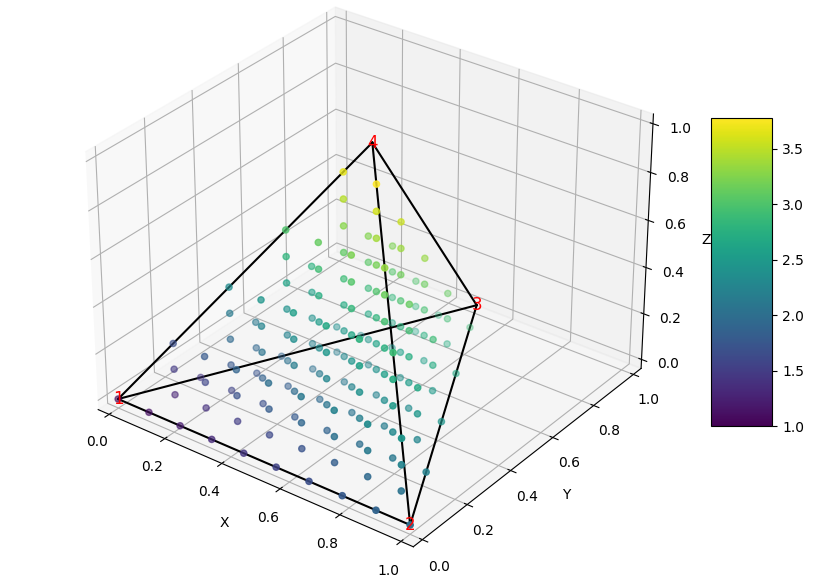
\includegraphics[width=\paperwidth,height=0.57\paperheight,
keepaspectratio]{images/Interpolation-quadratique-3D-thetraedre.png}}
}}}

\begin{document}

\AddToShipoutPicture*{\BackgroundPic}

\begin{titlepage}

    \changepage{3cm}%amount added to textheight
           {}%amount added to textwidth
           {}%amount added to evensidemargin
           {}%amount added to oddsidemargin
           {}%amount added to columnsep
           {-1.5cm}%amount added to topmargin
           {}%amount added to headheight
           {}%amount added to headsep
           {}%amount added to footskip

    
    \parindent=0pt
    
\includegraphics[scale=0.30]{images/ipsagarde.png} \hspace*{\stretch{1}}    
\includegraphics[scale=0.4]{images/cerfacsgarde.png}\\
    Institut Polytechnique \hspace*{\stretch{1}} Centre Européen de Recherche et de \\
    Des Sciences Avancées \hspace*{\stretch{1}}Formation Avancée en Calcul Scientifique\\
    81 Av. de Grande Bretagne \hspace*{\stretch{1}}Météopole 42 Av. Gaspard Coriolis\\
    31300 Toulouse \hspace*{\stretch{1}}31100 Toulouse
    \vspace*{1.5cm}
    \begin{center}
        \bfseries\LARGE Rapport de stage Aéro 4
    \end{center}
    \hrulefill
    \begin{center}\bfseries\huge
        Développement d'une méthode d'interpolation trilinéaire et évaluation de ses performances dans l'application de l'aéroacoustique
    \end{center}
    \begin{center}\huge
        Stagiaire au sein de l'équipe CFD
    \end{center}


    \vspace*{\stretch{2}}
    \begin{tabbing}
        Clément THIBAULT - Aéro 4 \= \hspace{6cm} \= Stage effectué du 10 juin 2024 \kill
        Clément THIBAULT - Aéro 4 \> \> Stage effectué du 10 juin 2024 \\
        Tuteur de stage : Carlos MONTILLA \> \> au 1 septembre 2024
    \end{tabbing}
    \vspace*{1cm}

% Bottom of the page

\end{titlepage}

\newpage
\pagenumbering{arabic}
\setcounter{page}{2}

\chapter*{Remerciements}

Je tiens à sincèrement remercier mon maître de stage Carlos pour m'avoir guidé tout au long de ce stage et toujours aidé avec le sourire.

\vspace{0.5cm}

Je tiens également à remercier Madame la présidente du CERFACS, Catherine LAMBERT, pour sa sympathie et pour m'avoir permis de faire ce stage. % pour sa bienveillance et pour m'avoir offert l'opportunité de réaliser ce stage.

Merci à amis montagnards et matheux Benjamin CANOVAS-ANDRIEUX et Dimitri LANIER ainsi que celle de mon professeur de mathématiques à l'IPSA, Guillaume COUFFIGAL, pour leurs précieuse aide en mathématiques.

Merci à mon tuteur pédagogique, Nadir MESSAI, pour son aide dans ma recherche de stage et au sein du CERFACS.

Merci à Alexis BOUDIN pour ses explications sur l'interpolation d'ordre élevé.
Je remercie mon ami, colocataire, collègue au CERFACS et à l'IPSA, Kélian RENOUX, Arthur COLOMBIÉ, Guillaume DAVILLER, l'administration, le CSG et Luc POTIER, mon cobureau, pour l'aide qu'ils m'ont apportée au CERFACS.




\vspace*{\fill} % Remplir l'espace vertical jusqu'en bas de la page
\begin{center}
    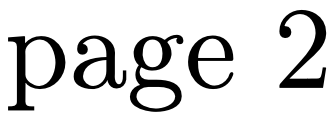
\includegraphics[width=0.067\textwidth]{images/page_2.png}
\end{center}
\vspace*{-13.5cm} % Ajustez cette valeur pour que l'image soit plus proche du bas de la page
\vspace*{\fill} % Remplir l'espace vertical après l'image


\newpage
\tableofcontents

\newpage
%\chapter{Bilan Technique}
\section*{Bilan Technique}
\addcontentsline{toc}{chapter}{Bilan Technique}
%\begin{comment}
Ce bilan technique a pour objectif de synthétiser les écarts et leurs causes entre les missions du stage et ce qui a été réalisé.
Il permet aussi de proposer ce qui pourrais être fait pas la prochaine personne travaillant sur le même sujet.

\begin{table}[ht]
\centering
\begin{tabular}{|p{6.5cm}|p{8.5cm}|}
\hline


\multicolumn{2}{|c|}{\textbf{Fiche de synthèse}   \hspace{7cm}   Clément THIBAULT - Aéro 4} \\ 
\hline
\textbf{Sujet de stage} & \textbf{Objectifs} \\ 
\hline


\begin{minipage}[t]{6.5cm}
Influence de la méthode d’interpolation sur la propagation acoustique FWH
\end{minipage} & 
\begin{minipage}[t]{8.5cm}
%\begin{itemize}
- Développer une méthode d’interpolation linéaire HPC dans Antares

- Évaluer l’influence de la méthode d’interpolation dans la qualité des résultats de propagation acoustique avec l’analogie FWH

- Améliorer les performances HPC de la méthode d’interpolation dans Antares
%\end{itemize}
\end{minipage} \\ 
\hline
\textbf{Client principal} & \textbf{Outils utilisés} \\ 
\hline
\begin{minipage}[t]{6.5cm}
%\begin{itemize}
- CERFACS

- Date de mise à jour : 15 octobre 2024
%\end{itemize}
\end{minipage} & 
\begin{minipage}[t]{8.5cm}
VSCode, Python, Kraken (supercalculateur du CERFACS), Antares, Paraview, Git
\end{minipage} \\ 
\hline
\multicolumn{2}{|l|}{\textbf{Études réalisées}} \\ 
\hline
\multicolumn{2}{|p{14cm}|}{
\begin{minipage}[t]{14cm}
\begin{itemize}
    \item Influence de paramètres de la méthode d'interpolation IDW
    \item Différences de DSP entre la méthode IDW et linéaire
    \item Optimisation de la rapidité du traitement
    \hspace{0.5cm}
\end{itemize}
\end{minipage}
} \\ 
\hline
\textbf{Résultats} & \textbf{Explications des écarts possibles} \\ 
\hline
\begin{minipage}[t]{6.5cm}
%\begin{itemize}
%\raggedright
%\justifying

- Meilleurs paramètres pour l'IDW se situent autour de N=10 et p=10

- Méthode linéaire généralement plus précise que IDW

- Rapidité du code d'interpolation augmentée, pour toutes les méthodes, d'un facteur 100 sur le cas test d'aéroacoustique

%\item Paramètres n \simeq 10 et p \simeq 10 optimaux pour la méthode IDW
%\end{itemize}
\end{minipage} & 
\begin{minipage}[t]{8.5cm}

- N=10 et p=10 donnent beaucoup d'information et d'importance aux points proches

- La méthode linéaire est d'ordre 1 contrairement à IDW qui n'a pas d'ordre au sens usuel du terme

- Pour la rapidité, une amélioration a consisté à ne pas recalculer des coefficients à chaque instant de la solution

\end{minipage} \\ 
\hline
\textbf{Difficultés rencontrées} & \textbf{Travaux à poursuivre} \\ 
\hline
\begin{minipage}[t]{6.5cm}
%\begin{itemize}
- Prise en main des outils

- Adapter la méthode linéaire au code déjà existant
%\end{itemize}
\end{minipage} & 
\begin{minipage}[t]{8.5cm}
%\begin{itemize}
- Optimiser la méthode linéaire pour les maillages prismatiques

- Traiter les maillages 'multi-zones' avec points partagés en linéaire

- Implémenter une méthode d'ordre supérieur

- Passer le code en parallèle pour améliorer la rapidité sur supercalculateur
%\end{itemize}
\end{minipage} \\ 
\hline
\end{tabular}
\end{table}  
%\end{comment}
\newpage

\newpage

%\chapter{Introduction}
\section*{Introduction}
\addcontentsline{toc}{chapter}{Introduction}

Ce stage de M1, d'une durée de trois mois, s'est déroulé au CERFACS, un institut reconnu pour son expertise en calcul \ac{HPC}. L'objectif principal était d'explorer et d'améliorer les méthodes d'interpolation dans le cadre du post-traitement de simulations numériques, avec un focus particulier sur l'application en aéroacoustique.

Le secteur de la recherche en calcul scientifique est réputé pour son environnement exigeant, mais stimulant, à la base de l'innovation. Le CERFACS, en particulier, est un acteur principal dans le domaine du HPC, collaborant avec de grands industriels et institutions pour développer des solutions à la pointe de la technologie.

%Ce rapport de stage a deux objectifs :

%D'une part permettre à l'IPSA, de m'évaluer (la structure et le contenu principal de ce rapport sont fixés par l'école).

%D'autre part fournir un rapport sur mon stage pour le CERFACS et pour d'autres personnes qui utiliseraient ou modifieraient le traitement d'interpolation d'Antares.

\vspace{0.5cm}

J'adore les mathématiques appliquées, la mécanique des fluides et je voulais découvrir le monde de la recherche. Lors d'une présentation des activités au \ac{CERFACS} par nos deux enseignants chercheurs Arthur COLOMBIÉ et Nadir MESSAI, j'ai eu l'occasion de découvrir ce laboratoire et d'y candidater pour mon stage de M1. Carlos MONTILLA, docteur au CERFACS, m'a proposé un sujet sur l'interpolation dans le cas de post-traitement de simulations numériques et son application en aéroacoustique. Le sujet m'a interpellé et c'est avec enthousiasme que j'ai ainsi pu commencer mon stage le 10 juin 2024 au CERFACS.

En quelques mots, le CERFACS est un institut de recherche privé, spécialisé dans le développement de code HPC, financé par sept actionnaires. %(voir ref \ref{actionnaires})

Antares\cite{antares} est un code d’analyse de données privé sous forme de librairie python, développé au CERFACS en 2012 et dont l'objectif est de réaliser du pré et post-traitement sur des simulations numériques utilisées par le CERFACS, ses actionnaires et autres partenaires.
Il contient notamment une fonction d'interpolation, codée en Python.

Mon maître de stage, Carlos MONTILLA, est responsable d'Antares depuis dix mois. Il a notamment fortement contribué au traitement \ac{FWH}. La chaîne de calcul aéroacoustique utilise le traitement d'interpolation avant de pouvoir utiliser le traitement FWH (voir Figure \ref{fig:chaineFWH}).

Mes missions principales lors de ce stage ont été :

- de faire un état des lieux sur les autres méthodes d'interpolation qui seraient 
implémentables dans Antares (avec les contraintes associées);
% A savoir, 3D, non structuré, temps de calcul, caractéristiques des équations à interpoler ...

- d'identifier les meilleurs paramètres pour l'équation \ac{IDW}, la seule qui était implémentée jusqu'alors dans Antares; % : Inverse Distance Weighting, pondération inverse à la distance en français}

- d'implémenter la méthode linéaire.  % \ac{DSP} à placer

\vspace{0,5cm}

Pour bien comprendre l'idée globale, l'objectif est d'interpoler les valeurs aux points d'un maillage 'cible', issu d'une discrétisation de l'espace, en utilisant les valeurs aux points d'un maillage 'source'.
Par exemple dans le cadre d'un raffinement de maillage entre deux itérations de calcul ou bien dans le cadre de la création d'une sphère dans un maillage 3D pour l'application des équations de FWH pour la propagation aéroacoustique.

\vspace{0,5cm}

Pour expliquer plus en détail ce stage au CERFACS, je présenterai dans une première partie ce laboratoire de recherche, puis dans une seconde partie j'exposerai le travail que j'ai réalisé sous forme de rapport. Cette seconde partie se décomposera en quatre temps : la présentation de la librairie Antares, les différentes méthodes d'interpolation, l'implémentation de la méthode linéaire dans Antares et finalement les tests de l'ancienne et de la nouvelle méthode.
\newpage

%\chapter{Présentation de l'entreprise}
\chapter{Le laboratoire de recherche CERFACS}
%\chapter{CERFACS : Le fondement des logiciels de simulation numérique}
%\chapter*{Le CERFACS : Le fondement des logiciels de simulation numérique}
%\addcontentsline{toc}{chapter}{Le CERFACS : Le fondement des logiciels de
                                %simulation numérique}

% Faire les sous parties


%Le plan doit être dynamique : le lecteur doit ressentir une progression entre le début et la fin du rapport. Ainsi, la « présentation de l’entreprise » (partie I) doit permettre de mieux comprendre la « présentation du travail réalisé » (partie II). En effet, les choix industriels, les processus de fabrication, les méthodes de travail, l’organisation et la culture de l’entreprise, notamment en matière de responsabilité sociétale et de développement durable (voir annexe IV, p. 39), ont nécessairement une incidence sur le travail
%du stagiaire.

Le CERFACS est un laboratoire de recherche privé dont les actionnaires sont Airbus, le CNES (Centre National d'Études Spatiale), EDF (Électricité de France), Météo France, l'ONERA (Office National d'Études et de Recherche Aérospatiales), Safran et TotalEnergies. Il a pour but de développer la simulation numérique par le calcul HPC pour ses actionnaires, mais aussi de faire de la recherche et de former des ingénieurs, chercheurs et doctorants. Il a été créé en 1988 sous le statut de \ac{GIP}, pour devenir une société civile en 1996 et depuis 2021, le CERFACS est une SAS (Société par Actions Simplifiées).

\vspace{0,5cm}

Les deux bâtiments du CERFACS sont situés au Météopole, dans la partie Ouest de Toulouse. Environ 170 personnes y travaillent, dont 20 \% de femmes, 50\% de doctorants et 20\% d'étrangers dont la moitié ne sont pas Européens.

% Budget environ 10M/an

Physiciens, mathématiciens, informaticiens, numériciens et data Scientist y travaillent dans cinq équipes :

% Tout en français OU tout en anglais

\begin{itemize}
    \item \ac{ALGO-COOP}
    \item \ac{CSG}
    \item \ac{ES}
    \item \ac{AAM}
    \item \ac{GLOBC}
\end{itemize}

\hspace{0,5cm}

% (Algorithmes Parallèles \& sCientifics sOftware Operational Performances)
% (Équipe Informatique et Support Utilisateur)
% (Energy et Safety)
% (Advanced Aerodynamics and Multiphysics)
% (Modélisation du climat et de son changement global)

La \ac{CAO} permet de faire les plans numériques d'un avion par exemple, afin de s'assurer que toutes les pièces fabriquées vont bien s'imbriquer entre elles. Mais cela permet aussi de faire des simulations numériques pour prévoir à l'avance la tenue structurelle, les forces aérodynamiques, le volume sonore, etc. sans avoir à faire d'onéreux tests.

L'équipe AAM se focalise sur la simulation des écoulements en développant des méthodes numériques avancées et en les appliquant aux avions, fusées, hélicoptères, moteurs, turbomachines, etc. Les liens de l’équipe AAM avec toutes les autres équipes du CERFACS sont forts, car ces équipes utilisent aussi la \ac{CFD} de façon intensive pour prévoir leurs modèles : en effet, derrière ces thèmes, on retrouve en premier les équations qui régissent les écoulements des fluides.

\hspace{0,5cm}

Le CERFACS héberge des supercalculateurs (Kraken et Calypso) et un serveur sur lequel se trouve l'intranet avec toutes les ressources nécessaires aux employés.
Nous y trouvons notamment les liens vers la \ac{QVT}, le \ac{CSE}, un document "Plan du management de la qualité" et énormément d'autres ressources.
%Le \ac{CSSCT} et le \ac{DUERP} devraient obligatoirement y être présents selon le site du gouvernement. % détailler







\newpage

Après une recherche non fructueuse sur l'intranet, j'ai pu demander à la responsable des ressources humaines le document relatant des objectifs \ac{RSE}. Le document d'actions RSE est segmenté en trois parties principales :

\paragraph{Démarche RSE}

%En voici le contenu :

\begin{quote}
\setlength{\leftmargin}{0.5cm} % Ajuster la marge gauche
\setlength{\rightmargin}{0.5cm} % Ajuster la marge droite
    "Le Cerfacs n’a pas mis en place une démarche spécifique RSE mais des actions ont été réalisées dans
    ce cadre, vis-à-vis de l’écoresponsabilité, la qualité de vie au travail et une charte éthique a été
    incluse dans le règlement intérieur depuis décembre 2023 (intégrant notamment la prévention de la
    corruption et la gestion des conflits d’intérêts).
    \hspace{0,5cm}

    En outre, le Cerfacs achète ses fournitures auprès de créateurs solidaires (exemple : Antilope qui
    compte 32 salariés sur les 49 avec une reconnaissance de « travailleur handicapé »).
    \hspace{0,5cm}

    Le Cerfacs met à jour au moins deux fois par an et aussi souvent que nécessaire un document unique
    d’évaluation des risques Cerfacs (avec un plan d’actions de prévention).
    \hspace{0,5cm}

    Le Cerfacs a nommé des référents : un référent « Santé et Sécurité », un référent « \ac{RGPD} », un
    référent « Handicap », deux référents « Harcèlement, agissements sexistes et violences ».

    Un bilan HSE et RSE est présenté chaque année aux Associés du Cerfacs lors de l’Assemblée d’avril."
\end{quote}



\paragraph{Écoresponsabilité}
\hspace{0,5cm}

    J'ai constaté beaucoup d'actions dans le sens de l'écoresponsabilité lors de mon stage. La plupart sont mentionnées dans le document d'actions RSE.
    \vspace{0,5cm}

    Un Groupe de Travail « Bilan carbone du CERFACS », composé de 10 volontaires, a été créé. Des bilans carbone ont été réalisés pour les années 2019 et 2021, en suivant la méthodologie proposée par le collectif de laboratoires Labos1point5\footnote{\url{https://labos1point5.org}}. Depuis mi-2023, le CERFACS collabore avec le Cabinet Take[air] pour établir un plan d’actions visant à réduire son empreinte carbone. Cette collaboration a permis de réaliser le bilan carbone de 2022 et de commencer l'élaboration d'un plan d'actions, qui devrait être finalisé à l’automne 2024, après la tenue de plusieurs ateliers. Finalement nous trouvons dans le document un tableau\ref{tab:Eco_actions} récapitulant les principaux postes d'émission identifiés dans une première colonne puis les objectifs et actions associés dans une seconde colonne.

    En parallèle, j'ai entendu parler de cette démarche en discutant avec des thésards. Et j'ai aussi pu trouver la page depuis l'intranet. Elle est divisée en cinq sections : "présentation", "actualités", émissions", "bilan" et "actions".
    J'aime beaucoup l'image ci-dessous, présente dans le document et le site internet, qui montre que le CERFACS réduit ses émissions d'année en année, probablement grâce aux efforts du groupe « Bilan carbone du CERFACS »  : 

    \begin{figure}[H]
        \centering
        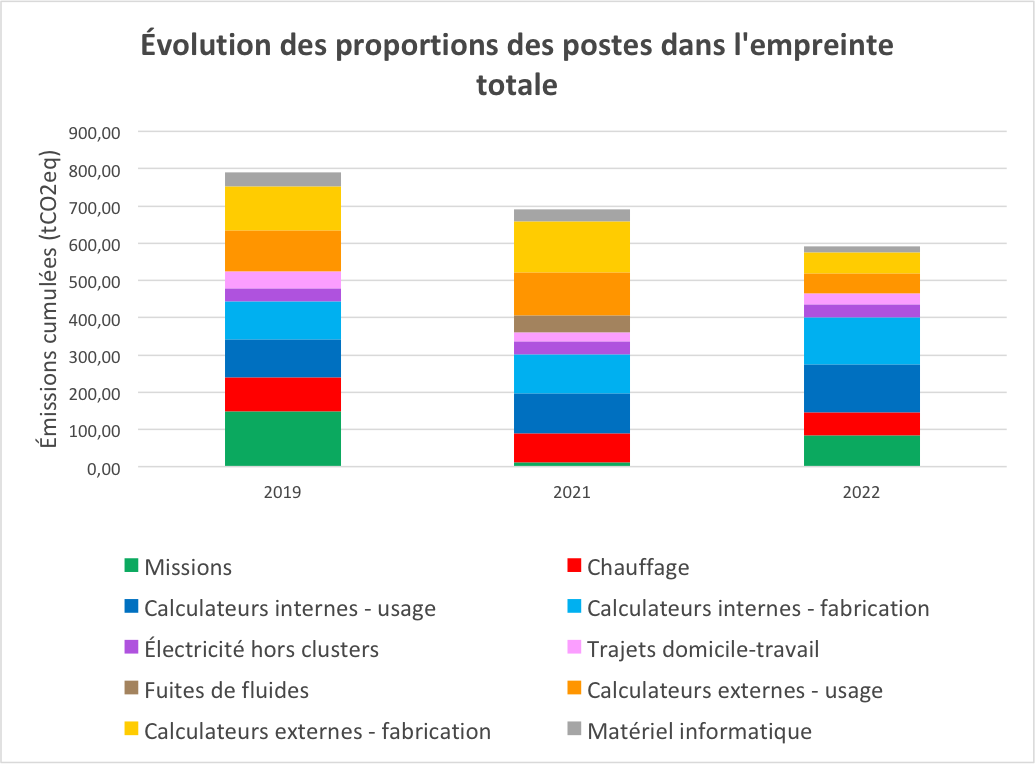
\includegraphics[width=0.85\textwidth]{images/evolution_postes_empreintecarbone.png}
        \caption{Evolution de l'empreinte carbone du CERFACS entre 2019 et 2022}
    \end{figure}

    Dans les couloirs du CERFACS on trouve des posters très clairs sur l'empreinte carbone d'un trajet pour une conférence en fonction des moyens de transports.

    Les employés sont incités à venir à vélo. Le CERFACS donne une prime pour chaque kilomètre fait à vélo sur le trajet habitation-travail-et vis-versa. Il y a aussi un atelier de réparation et des emplacements sécurisés pour les vélos.

    La politique de communication n'est pas spécialement tournée vers les efforts pour le climat ou la RSE, mais le CERFACS agit efficacement en ce sens.

\paragraph{Responsabilité sociale / Qualité de vie au travail}
\hspace{0,5cm}

    \begin{quote}
        \setlength{\leftmargin}{0.5cm} % Ajuster la marge gauche
        \setlength{\rightmargin}{0.5cm} % Ajuster la marge droite
        "La démarche Qualité de Vie au Travail (QVT) a été lancée au Cerfacs en janvier 2022, avec la mise en
        place d’un Groupe de Travail : elle a permis d’identifier 6 axes de travail pour améliorer le
        fonctionnement de la structure et du ressenti des personnes :
        \begin{itemize}
            \item Optimiser l’organisation et gestion du travail au niveau global
            \item Optimiser l’organisation et gestion du travail au niveau de l’équipe
            \item Optimiser l’organisation et gestion du travail au niveau personnel
            \item Assurer un meilleur accueil et support des non permanents
            \item Favoriser la vie sociale
            \item Améliorer le confort matériel"
        \end{itemize}
    \end{quote}

    De nouveau, un tableau\ref{tab:QVT_actions} détaille des exemples d'actions que j'ai pu experimenter (salle de repos, machine à café, endroit pour attacher son vélo, \dots)

    Un dernier plan d'action a été mis en place sur l'égalité professionnelle entre les femmes et les hommes. Il traite de diverse sujets : l’embauche, la rémunération effective et l’articulation entre l’activité professionnelle et l’exercice de la responsabilité familiale.

    Je tiens à mentionner également que j'ai reçu un mail qui lançait un appel au volontariat pour composer le Comité de Pilotage pour la Prévention des Violences Sexistes et Sexuelles au Travail suite à une réunion d'information réalisée en collaboration avec la médecine du travail.

\newpage


Mon ressenti personnel sur le cadre de travail est très positif. Être assis dans un bureau climatisé avec une vue sur la campagne participe évidement à cela. Un des seuls risques à ce type de travail est une mauvaise position qui peut entraîner des problèmes de dos, épaules, etc. Pour palier cela il y a des affiches dans chaque bureau indiquant la meilleure position à avoir et proposant des exercices. Ces mêmes informations apparaissent dans le 'livret d'accueil stagiaire' qui m'a été remis le premier jour.

Une cantine présente sur le site à quelques minutes à pied, permet de déjeuner et échanger avec les collègues du CERFACS hors cadre professionnel.
\newpage

%\chapter{Présentation du stage}
\chapter{Présentation du stage}

Mon stage a commencé le lundi 10 juin 2024. Après avoir récupéré un ordinateur et un PIN-pad générateur d'OTP (One-Time-Password), Carlos, mon maître de stage a pu me montrer comment comprendre la librairie que j'allais développer : Antares. Une ressouce sur l'intranet ? permet d'apprendre à l'utiliser. Pour vous illustrer la base d'une solution CFD que nous pourrions vouloir traiter avec Antares, voici un schéma :

\begin{figure}[ht!]
    \centering
    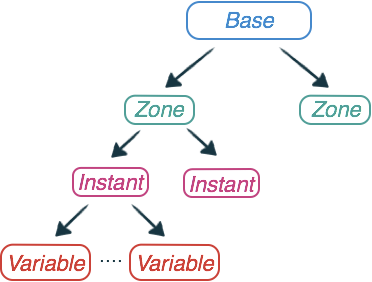
\includegraphics[width=0.5\textwidth]{images/data_structure_1.png}
    \caption{Structure des données} %\footnote{Source:https://cerfacs.fr/antares/src/tutorial/base.html}}
    %\label{fig:https://cerfacs.fr/antares/src/tutorial/base.html}
\end{figure}


Ensuite, j'ai été chargé de résoudre un petit bug sur Antares, ce qui m'a permis de prendre la main sur Nitrox, le gitlab hébergé sur le serveur du CERFACS où se situe Antares et d'autres codes du CERFACS.

\section{Mission 1 : Recherche les différentes méthodes d'interpolation}
Ma première mission a été de recensser les méthodes d'interpolation qui seraient implémentables dans Antares, à savoir, qui permettent de l'interpolation 3D, sur des maillages dits non structuré, c'est à dire pas de simples maillages, rectangulaires en 2D et hexaédrique en 3D, représentés par des matrices, mais des maillages créés avec différentes formes géométriques.
Le temps de calcul, appelé 'coût' est aussi un paramètre à prendre en compte.
Finalement, les caractéristiques des équations à interpoler est probalement le paramètre le plus important à prendre en compte mais aussi assurément le plus difficile. Effectivement différentes équations très difficiles à caractériser tel que l'équation de Naviers-Stokes sont utilisées et mon niveau en maths est trop limité pour pouvoir me plonger en profondeur dans ce problème. C'est pour cela que je n'ai pas de résultat mathématique à présenter dans cette partie. Mais heuresement que ces méthodes ont déjà été implémentés et testés pour d'autres codes de simulation numérique, ce qui donne une bonne idée des résultats que nous pouvons espérer.

%\addcontentsline{toc}{section}{L'interpolation et l'aéroacoustique}

\subsection{L'interpolation par voisin le plus proche}
Cette première méthode est très simple : nous prenons comme valeur \( v \) d'interpolation au point \( p \) la valeur \( v \) du point le plus proche de \( p \).
Nous comprenons assez vite que cette méthode est discontinue et même pas linéaire...
Nous pouvons aussi imaginer que 2 points à droit et à gauche d'une ligne horizontale de 3 points (les plus proches), prendrons la même valeur pour \( N \) = 3, Schématiser. 

D'autres méthodes dérivés ou similaiers existent pour évaluer nos poids. La plus intéressante serait celle dite de Franke-Littke. Elle consiste à utiliser une distance maximal autour du points au-delàs les autres points ne sont pas pris en compte. Autrement dit, en utilisant un cercle (dans le cas 2D) d'un certain rayon pour déterminer quels points nous sont utile pour l'interpolation. Dans ce cas le nombre de points est variable.
J'ai considéré subjectivement que cette méthode n'étais pas intéressante car, confronté à un maillage ayant une différence de rafinement intrinsèque importante, dans certains cas aucuns points ne seraient pris, et dans d'autes, une grande somme serait calculée.


\begin{comment}
Certaines conditions de cette méthode doivent être respectés, comme Pour N tends vers l’inf, p doit être inférieur ou égale à la dimension, par ex 3 pour ne pas diverger. Mais N n’est pas grand dans notre cas.
Voir d'autres choses page 7 de mon ppt.
\end{comment}


\subsection{L'interpolation IDW}
\[
\hat{f}(x) = \frac{\sum_{i=1}^{N} \frac{f(x_i)}{d(x, x_i)^p}}{\sum_{i=1}^{N} \frac{1}{d(x, x_i)^p}}
\]

où :

- \(\hat{f}(x)\) est la valeur interpolée à la position \(x\),

- \(f(x_i)\) est la valeur connue aux points de données \(x_i\),

- \(d(x, x_i)\) est la distance entre \(x\) et \(x_i\),

- \(p\) est le paramètre de puissance,

- \(N\) est le nombre total de points de données.



Probablement l'iterpolation la plus simple après la méthode du voisin le plus proche (toujours dans notre cas d'application), cette méthode est la seule qui étais implémenté dans Antares.

Nous pouvons modifier 2 paramètres : \(p\) et \(N\).
Par défault, dans le code, \(p\) = 1 et \(N\) est égale aux nombres de sommets de la première forme de cellule de la liste de formes de cellules de la base target (je n'ai pas compris pourquoi pas de la base source) /! Tests à faire ici /!
Ces informations ne sont pas confidentielles Carlos ?

Nous remarquons que pour \( n = 1 \), nous retrouvons la méthode du voisin le plus proche, pour tout \( p \).

Une de mes mission étais de chercher s'il y avait des paramètres plus optimisés que \(N\) et \(p\) pour cette méthode. Je n'ai pas trouvé le réponse dans les différents articles et thèses que j'ai lu. C'est pour celà que je présenterais plus tard comment j'ai trouvé des paramètre optimaux en faisant des tests.


\subsection{L'interpolation polynomiale}
\subsection{L'interpolation par Splines}
\subsection{Méthodes géostatiques}
\subsection{Méthode par moindres carré}
\subsection{MISCOG}

\subsection{L'interpolation linéaire}
Aussi appelée interpolation Barycentrique, l'inerpolation linéaire, est la plus simple (après les plus proches voisins et IDW), et la plus utilisée par Aibus, Safran et d'autres industriels (dans via d'autres codes qu'Antares).
C'est pour cela qu'ils ont demandé au CERFACS de l'implémenter des Antares, car ils l'utilisent actuellement via d'autres moyen.
En 1D, l'interpolation linéaire est simple : c'est la moyenne pondérée linéairement par la distance, des valeurs des points.
Supposons que nous voulons interpoler une valeur d'un point \( p \) entre deux points \( a \) et \( b \) dans un espace 1D
et que nous représentons leurs valeurs dans une deuxième dimension \( y \).
Nous aurons alors pour formule :

\[
y_p = \frac{x_b - x_p}{x_b - x_a} \cdot y_a + \frac{x_p - x_a}{x_b - x_a} \cdot y_b
\]

%\vspace*{0.1\baselineskip}\linebreak
où \( y_p \) représente la valeur interpolée à la position \( x_p \), et \((x_a, y_a)\) et \((x_b, y_b)\) sont les points de référence. J'ai écris cette formule afin qu'elle soit symétrique par rapport aux points \( a \) et \( b \), pour qu'il jouent la même rôle. Ainsi elle s'entendra plus intuitivement dans des dimensions supérieurs.
\vspace{0.5cm}
%\vspace*{0.1\baselineskip}\linebreak

        \( \frac{x_b - x_p}{x_b - x_a} \) est le poids pour \( y_a \) basé sur la distance relative de \( x_p \) à \( x_b \).

        \( \frac{x_p - x_a}{x_b - x_a} \) est le poids pour \( y_b \) basé sur la distance relative de \( x_p \) à \( x_a \).\vspace{0.5cm}

Ces deux termes sont pondérés de manière à ce que leur somme soit toujours égale à 1, ce
qui garantit que l'interpolation est correcte et symétrique par rapport à \( a \) et \( b \).\vspace{0.5cm}

En 2D, nous devons nous baser sur des surfaces, extraites de formes pour pouvoir effectuer cette pondération. En CFD, ces formes sont appelés cellues et leurs sommets noeuds. Dans notre cas, nous considérons que les variables du maillages sont contenus au niveau des noeuds. Aussi, Antares ne traites que des maillages ayant des valeurs uniquement au niveau des noeuds des cellules (pas entre).
Il existe 23 principales types de cellules (formes) en 2D : les triangles 'tri', et les quadrilatères 'qua' (non croisés) et les rectangles des maillages structurés.
Pour le triangle, la méthode pour trouver la valeur au point à interpoler \( p \) est celle dite du barycentre (barycentrique).
Elle est bien documentée. Visuellement, il faut faire la somme des valeurs au points pondéré par la surface opposé et pondéré le tout par la surface du triangle.

En ce qui concerne l'interpolation sur un rectangle, nous la trouvons aussi facilement. La formule est l'extension de celle pour les triangles :

EQUATION

Visuellement nous créons cette fois des traits parallèles au passant par le point d'interpolation et nous additionnons, de manière pondérée, les 4 surfaces multipliés chacune par leurs sommet opposé respectif. Cela correspond à deux interpolations linéraires. Souvent nous trouvons une équation analytique où tous les sommets ne jouent pas le même rôle mais je trouvais cela plus simple de faire un calcul de poids pour pouvoir ensuite faire une moyenne pondérée :

ILLUSTRATION

Viens maintenant la denière forme 2D rencontrée dans les solutions traités par Antares : les 'qua'. Pour celà je n'ai pas touvé de méthode. Après plusieurs essais sur papier, je me suis concenté sur le fait que la méthode devais être continue, ce qui implique notament que la valeur du point à interpoler doit tendre vers la valeur d'un sommet lorsque sa distance à ce dernier tend vers 0. Une première verification de la linéarité est aussi de vérifier qu'un point au milieu d'une forme 2D a comme valeur la moyenne de ses cotés.
Via cette démarche, j'ai imaginé, graphiquement, tracer des traits entre le point à interpoler et les sommets de la forme dans laquelle il se situe (tel que pour l'interpolation Barycentrique). Cela permet de ne créer uniquement 4 sous formes. Ensuite pour déterminer le poids associé au sommet \( s_1 \), il faut multiplier les deux surfaces qui lui sont opposés entre elles, et bien entendu, le pondéré une fois les autres poids calculés. Par opposé j'entends que ces surfaces ne sont composés d'aucune arrête ayant pour l'une de leurs extrémité le point d'interpolation. Ceci est important pour le 3D. Pour l'instant je n'ai démontré que par l'expérimentation que cette méthode étais linéaire. Un point qui me perturbais étais de faire des multiplications de sufaces, donc ordre 4, dans une méthode linéaire. Mais contrairement à son nom, l'interpolation bilinéaire est en réalité quadratique avec un résulatat linéaire. On pourrais imaginer que, par chance, ma méthode soit quadratique. Premièrement j'ai vérifier et ce n'est apparament pas le cas. Deuxièmement je pense que le quadratique n'englobe pas le linéaire dans la cas où nous nous basons uniquement sur les quatre points d'un quadrilatère. Effectivement, en 1D, si nous avons \(f(x_i)\) = 0 et \(f(x_{i+1})\) = 1, le résultat d'une variable linéaire serait 0,5 et celui d'une variable quadratique 0,25, si nous avons uniquement conaissance de ces deux points. Finalement voici l'équation :\\
EQUATION

ILLUSTRATION\vspace{0.5cm}  % OU \\[0pt plus 1fill] OU \newline OU flushleft, flushright, center

Pour le 3D, si le maillage est structuré, alors la forme est le pavé droit. A ce moment nous sommes dans le cas de l'interpolation dite trilinéaire. Encore une fois la formule se trouve facilement. Nous associons comme poid à un des huit sommet \( s_1 \) le volume opposé, construit de la sorte :

\begin{figure}[ht!]
    \centering
    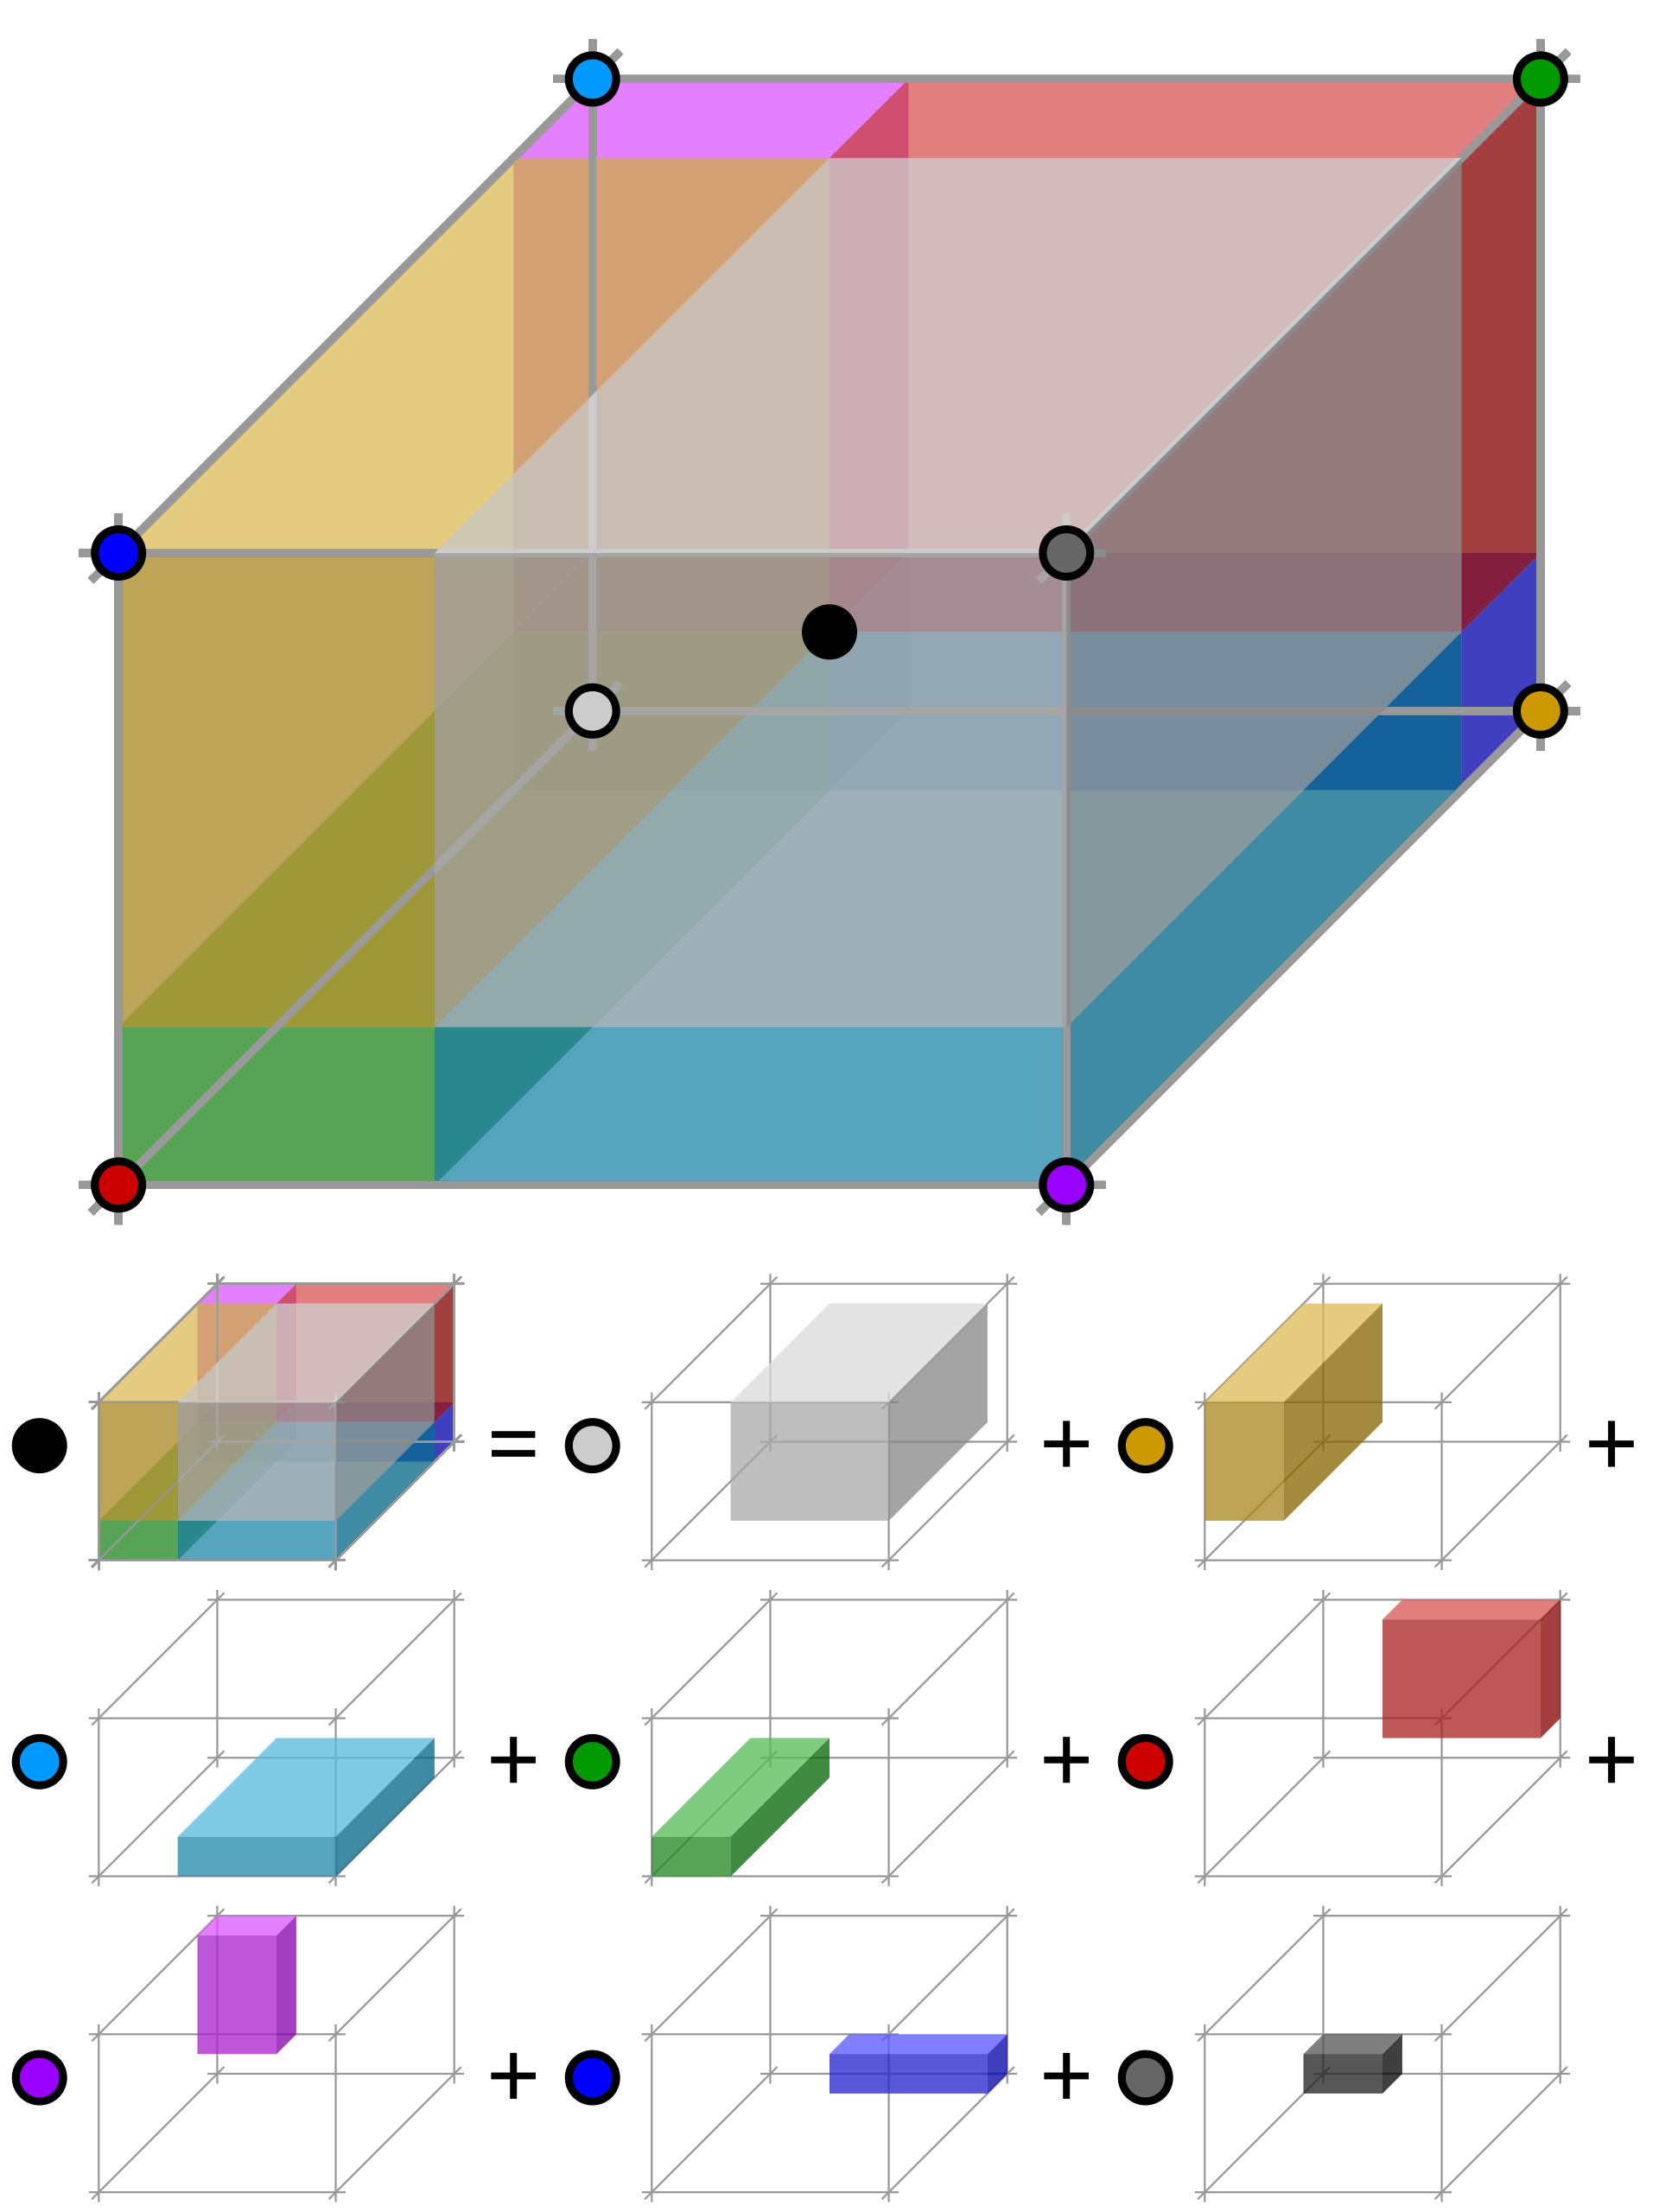
\includegraphics[width=0.4\textwidth]{images/Trilinear_interpolation_visualisation.svg.png}
    \caption{Interpolation trilinéaire} %\footnote{Source:https://en.wikipedia.org/wiki/Trilinear_interpolation#/media/File:Trilinear_interpolation_visualisation.svg}}
    %\label{fig:https://en.wikipedia.org/wiki/Trilinear_interpolation#/media/File:Trilinear_interpolation_visualisation.svg}
\end{figure}

L'équation qui en découle est la suivante :

\begin{equation}
    f(x, y, z) = \sum_{i=0}^{1} \sum_{j=0}^{1} \sum_{k=0}^{1} f_{ijk} (1 - |x - x_i|)(1 - |y - y_j|)(1 - |z - z_k|)
\end{equation}

% Expliquer mathématiquement ? Ou plus tard dans le code ?  (quadrilatère non croisé, concave et convexes)

% En CFD il y a toujours des formes, même si c'est structuré, on peut unstructure.

\subsection{Resumé des similitudes et différences des différentes méthodes}



\section{Mission 2 : Implémenter la méthode trilinéaire}
\subsection{La structure générale du code TreatmentInterpolation}
Après avoir recensé les différentes méthodes qui seraient applicables, ma seconde mission a été d'implémenter une interpolation linéaire dans Antares. Grace à Nitrox, j'ai accès au code source de la librairie que je peux modifier. Le code 'interpolation.py' faisais environ 500 lignes. Il est orienté objet. Il prend comme arguments obligatoires la base source et la base target et renvoie dans le cas le plus simple la base target avec les valeurs interpolés.
De manière simplifiée, dans le code, les zones de la base source sont fusionnées puis nous parcourons les instants. 
Cette fusion permet de faire un KDTree (pour arbre à k-dimensions), qui permet concrètement de rechercher de manière efficace quels sont les \( N \) points de la base source les plus proches des points de la base target (et les distances associés, utilisés dans la méthode 'idw').

Ensuite nous calculons l'interpolation via une méthode 'principale' (\lstinline{__idw_interpolate_instant} ou
\lstinline{__barycentrique_interpolate_instant}) qui peut elle-même appeler des fonctions ou méthodes.

\subsection{L'algorithme}
Si vraiment ce n'est pas confidentiel je peux mettre le code en annexe Carlos.

Premièrement, dans \lstinline{__barycentrique_interpolate_instant}, nous récupérons le nombre de points maximal sur lequel nous allons nous appuyer pour l'interpolation, soit le nombre maximale de sommet des formes présentes dans le maillage.
Nous récupérons les distances et le indices du KDtree.
Ensuite nous devons réarranger des indices qui se sont fait déplacer lors de la fusion des zones.
Nous récupérons aussi différentes variables, comme les coordonnées des points, \dots

Nous récupérons d'une fonction définie plus bas (\lstinline{get_list_cell_type}) :
(\lstinline{list_cell_type, max_node_index})


Dans le cas où le maillage est le même entre tous les instants, nous ne recalculons pas tout ces paramètres, ce qui permet une diminution significative du temps de calcul.


Expliquer 'is point on cell', etc...


%\subsection{La prise en main de la libraire Antares}
\subsection{...}

EXEMPLE DE MISE EN FORME PYTHON
\begin{lstlisting}[caption=Calcul de l'interpolation, label={lst:interpolation}]
    def __idw_interpolate_instant(x, y, z, values, power=2):
        # Calculer l'interpolation IDW
        weights = [(1 / (distance**power)) for distance in distances]
        interpolated_value = sum(w * v for w, v in zip(weights, values)) / sum(weights)
        return interpolated_value
    
    def __barycentrique_interpolate_instant(x, y, z, values):
        # Calculer l'interpolation barycentrique
        weights = [barycentric_weight(x, y, z, vertex) for vertex in vertices]
        interpolated_value = sum(w * v for w, v in zip(weights, values))
        return interpolated_value
\end{lstlisting}


\subsection{Les difficultés}
\subsection{Le résultat}



\section{Mission 3 : Tester sur des cas d'aéroacoustique}
% \section{Les différentes méthodes d'interpolation}
Carlos a développé l'outils permettant de déterminer le résultat acoustique, à grande distance, à partir d'un surface, en utilisant les équations de Ffowcs Williams – Hawkings. Le résultat acoustique sont les petites variations de pression, impliquant du son (à différentes fréquences et amplitudes). En pratique, pour les utilisateurs d'Antares, cette surface est définie dans un maillage 'solution' où nous avons le résutlat de la pression en différents points et différents instants.
% Paramètres d'IDW
\subsection{Tests sur les paramètrs de la méthode IDW}




... (\url{https://cerfacs.fr/antares/}) : 


\begin{itemize}
    \item TreeMesh 
    %Ici, le maillage DGMultiMesh dépend directement du solver DGMulti en fonction du type de géométrie utilisée, il faut donc le passer en argument.
\end{itemize}


\subsection{Discrétisation spatiale et résolution du problème}
\newpage

%\chapter{Conclusion}
\chapter*{Conclusion}
\addcontentsline{toc}{chapter}{Conclusion}

%L'objectif de ce stage était d'implémenter une méthode d'\textbf{interpolation linéaire} dans \textbf{Antares} puis de comparer sa précision avec la \textbf{méthode IDW} dans le cas de propagation acoustique avec l'analogie FWH, tout en optimisant la vitesse d'exécution du code.
%Premièrement, une recherche documentaire sur les méthodes d'interpolation implémentables dans notre cas a été menée.
%Ensuite, la méthode linéaire a été implémentée en utilisant une méthode particulière pour les cellules non triangulaires ou rectangulaires.
%L'efficacité a été augmentée dans les cas multi-instants partagés en évitant le recalcule des coefficients d'interpolation à chaque itération. Ces mêmes coefficients peuvent être récupérés par l'utilisateur qui voudrait appeler deux fois le traitement pour une base ayant une même structure.
%La méthode linéaire a été testée sur des cas simples et industriels. Elle fonctionne correctement sur tous les types de cellules, sauf dans certains cas très complexes comme des prismes ayant des faces opposées de tailles différentes et/ou non parallèles.
%Dans le cas de l'aéroacoustique, la méthode linéaire est plus précise que IDW dans tous les cas testés. Cependant, des résultats expérimentaux ont montré que des coefficients (\(N\), \(p\)) autour de (10, 10) donnaient de très bons résultats. Dans ce cas, IDW peut s'avérer plus précis que la méthode linéaire.
\subsection*{Bilan technique et humain}

Ce stage au CERFACS m'a vraiment plu. Il m'a permis de développer et renforcer beaucoup de connaissances dans le milieu de l'informatique, mais aussi sur le plan humain. J'ai pu découvrir comment se déroulait la vie en laboratoire de recherche.

L'objectif de ce stage était d'implémenter une méthode d'interpolation linéaire dans Antares puis de comparer sa précision avec la méthode IDW dans le cas de propagation acoustique avec l'analogie FWH, tout en optimisant la vitesse d'exécution du code.
Après avoir exploré la structure d'Antares, une recherche documentaire a été menée pour savoir quelle méthode, implémentable dans la librairie, pouvait être candidate pour compléter la méthode idw et linéaire. Quelques méthodes polynomiales et géostatistiques en sont ressorties. Une présentation un plus détaillé de la méthode par voisin le plus proche, IDW et linéaire a aussi été réalisé.
L'un des principaux résultats de ce stage a été l'implémentation globalement réussie de la méthode d'interpolation linéaire, qui s'est avérée généralement plus précise que la méthode de Pondération Inverse à la Distance (IDW) précédemment codée.
Coder l'interpolation linéaire jusqu'en 3D n'a pas été très difficile ou chronophage, mais bien l'intégrer au code déjà existant et faire les tests l'était plus. Le soutien de mon maître de stage a été primordiale pour me montrer comment fonctionne les outils au CERFACS, me débloquer, etc.
Cette nouvelle méthode a été testée sur des cas académiques comme sur des cas industriels comme sur une vue en coupe à la position (0, 0, 0.01), selon l'axe z de la chambre de combustion preccinsta.
L'étude sur les coefficients \(N\) et \(p\) de la méthode IDW a montré que pour des paramètres (\(N\), \(p\)) autour de (10, 10) nous pouvons obtenir de meilleurs résultats que la méthode linéaire, dans le cas d'aéroacoustique étudié.
Ce travail aussi amélioré les performances du code (cinq fois plus rapide pour la méthode IDW dans un cas test d'aéroacoustique).
Le code ajouté pourrait aussi aider à l'intégration de méthodes d'ordre supérieur grâce à certaines fonctions python réutilisables.
J'ai ressenti tout au long de mon stage l'importance de faire un travail qui puisse être continué plus tard par un autre chercheur.
Enfin, ce stage a été une expérience enrichissante qui a conforté mon intérêt pour les méthodes numériques appliquées et la recherche en calcul scientifique. Je suis reconnaissant pour l'accompagnement que j'ai reçu tout au long de cette expérience et pour les opportunités de développement personnel et professionnel qu'elle m'a offert.

\subsection*{Perspectives}
Pour continuer à améliorer le traitement d'interpolation d'Antares, on pourrait implémenter l'une des méthode d'ordre supérieur cités dans la section \ref{s223}.
Afin d'améliorer la rapidité, le code pourrais être passé en parallèle pour pouvoir s’exécuter sur plusieurs processeurs à la fois.
Une petite amélioration qui permettrait de rendre le code compatible avec plus de base serait d'inclure les bases 'multi-zones'à l'interpolation linéaire.
% Faire la ref


\subsection*{Réflexion personnelle}

Le CERFACS est un laboratoire privé à la points des simulations numériques. Il s'est d'abord spécialisé dans l'aérodynamique et s’intéresse maintenant de plus en plus à la combustion. Il adapter ses domaines de recherche vers les domaines importants de l'industrie.
Durant ce stage, au-delà des aspects techniques, j'ai eu un bel aperçu du métier de chercheur tant au travers de mes missions que dans mes rencontres. Il s'agit de rechercher et de s'appuyer sur le travail déjà réalisé autour de notre problématique. Ensuite, il faut essayer des pistes qui peuvent s'avérer infructueuses après les avoirs longuement explorés. Finalement un travail de rédaction est nécessaire pour expliquer clairement notre travail à la science.

\newpage

%\chapter{Annexes}
\section*{Annexes}
\addcontentsline{toc}{chapter}{Annexes}


\counterwithin{table}{section}
\counterwithin{figure}{section}
\counterwithin{table}{section}

\renewcommand{\thetable}{A\arabic{table}}
\renewcommand{\thefigure}{A\arabic{figure}}
\setcounter{figure}{0}

%\section{Détails des objectifs et actions liées à l'écoresponsabilité}

% Chaque annexe porte un numéro et un titre.

\begin{table}[H]
    \centering
    \begin{tabular}{|p{4,5cm}|p{10,5cm}|}
    \hline
    \textbf{Les principaux postes d’émissions identifiés} & \textbf{Quelques objectifs et actions} \\
    \hline
    Missions & 
    - Prévention sur le sujet sur le site Carbon Footprint du Cerfacs et affiches présentes dans les locaux. \\
    \hline
    Chauffage & 
    - Rénovation du circuit d’alimentation en eau glacée des ventilo-convecteurs de l’ancien bâtiment (Actions 2023 et 2024) \newline
    - Traitement de l’étanchéité et de l’isolation de l’ancien bâtiment (analyse réalisée, actions en cours réparties sur plusieurs années pour cause de coût global). \\
    \hline
    Calculateurs internes et usage & 
    - Un calculateur a été arrêté en février 2023 et remplacé seulement en 2024. \newline
    - Une sensibilisation à l’optimisation de l’usage des calculateurs \\
    \hline
    Calculateurs internes et \\fabrication & 
    \phantom{-}
    \phantom{-}\\
    \hline
    Électricité hors clusters & 
    - Automatisation de l’éclairage des circulations de l’ancien bâtiment (abandon de l’éclairage manuel). \\
    \hline
    Trajet domicile-travail & 
    - Participation à des initiatives en faveur du vélo ("Deux Pieds Deux Roues - 2P2R", "Objectif Employeur Pro Vélo") \newline
    - Mise en place du Forfait Mobilité Durable pour le vélo. \newline
    - Mise à disposition de deux vélos pour le personnel du Cerfacs \\
    \hline
    Fuites de fluides &  \\
    \hline
    Calculateurs externes et usage & 
    - Une sensibilisation à l’optimisation de l’usage des calculateurs \\
    \hline
    Calculateurs externes et \\fabrication &
    \phantom{-}
    \phantom{-}\\
    \hline
    Matériel informatique & 
    Les postes de travail sont globalement à jour et ont un bon niveau de technologie (77\% publiés en 2023). \\
    \hline
    \end{tabular}
    \caption{Axes de travail et exemples d'actions pour limiter l'empreinte carbone du \\ CERFACS}
    \label{tab:Eco_actions}
\end{table}


%\section{Détails des actions liées à la Qualité de Vie au Travail}

\begin{table}[H]
    \centering
    \begin{tabular}{|p{5cm}|p{10cm}|}
    \hline
    \textbf{Axes de travail} & \textbf{Exemples d’actions} \\
    \hline
    Optimiser l’organisation et gestion du travail au niveau global & 
    - Organisation d’une réunion générale du Cerfacs par la direction 2 fois par an \newline
    - Valorisation de la bibliothèque (réaménagement de l’espace) \newline
    - Amélioration de la communication interne (journal de la QVT disponible sur l’intranet, newsletter interne mensuelle) et externe (nomination d’un référent Communication) \\
    \hline
    Optimiser l’organisation et gestion du travail au niveau de l’équipe & 
    - Proposer une formation à l’organisation et à la tenue de réunions efficaces \\
    \hline
    Optimiser l’organisation et gestion du travail au niveau personnel & 
    - Information/sensibilisation au burn-out (par la médecine du travail) \\
    \hline
    Assurer un meilleur accueil et support des non permanents & 
    - Mise en place d’un groupe de travail pour optimiser l’encadrement des non-permanents (doctorants, post-doctorants…) \newline
    - Rédaction d’une charte QVT \\
    \hline
    Favoriser la vie sociale & 
    - Organisation d’événements sociaux en dehors du temps de travail \newline
    - Aménagement d’une salle de repos \newline
    - Organisation de pauses café collectives mensuelles \\
    \hline
    Améliorer le confort matériel & 
    - Nouvelle machine à café à grain mise à disposition pour tous (avec l’achat de café par le Cerfacs) \newline
    - Gourdes métalliques offertes à l’ensemble du personnel \newline
    - Achat et installation de nouveaux arceaux pour augmenter la capacité d’accueil des vélos \newline
    - Sensibilisation à l’ergonomie sur le poste de travail (par la médecine du travail) \\
    \hline
    \end{tabular}
    \caption{Axes de travail et exemples d'actions pour la Qualité de Vie au Travail au CERFACS}
    \label{tab:QVT_actions}
\end{table}


\begin{figure}[H]
    \centering
    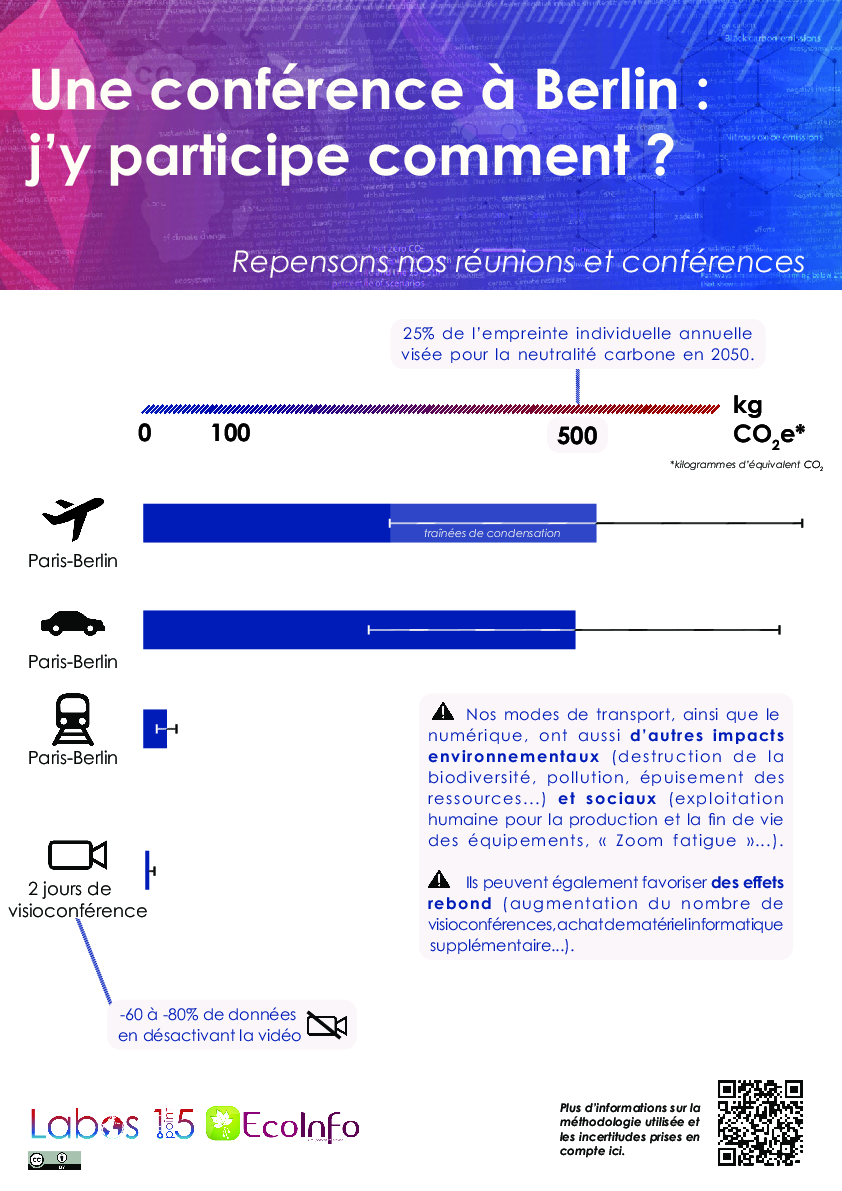
\includegraphics[width=0.5\textwidth]{images/berlin_v7_fr.png}
    \caption{Empreinte carbone s'une conférence à Berlin}
    \label{fig:berlin}
\end{figure}

\begin{figure}[H]
    \centering
    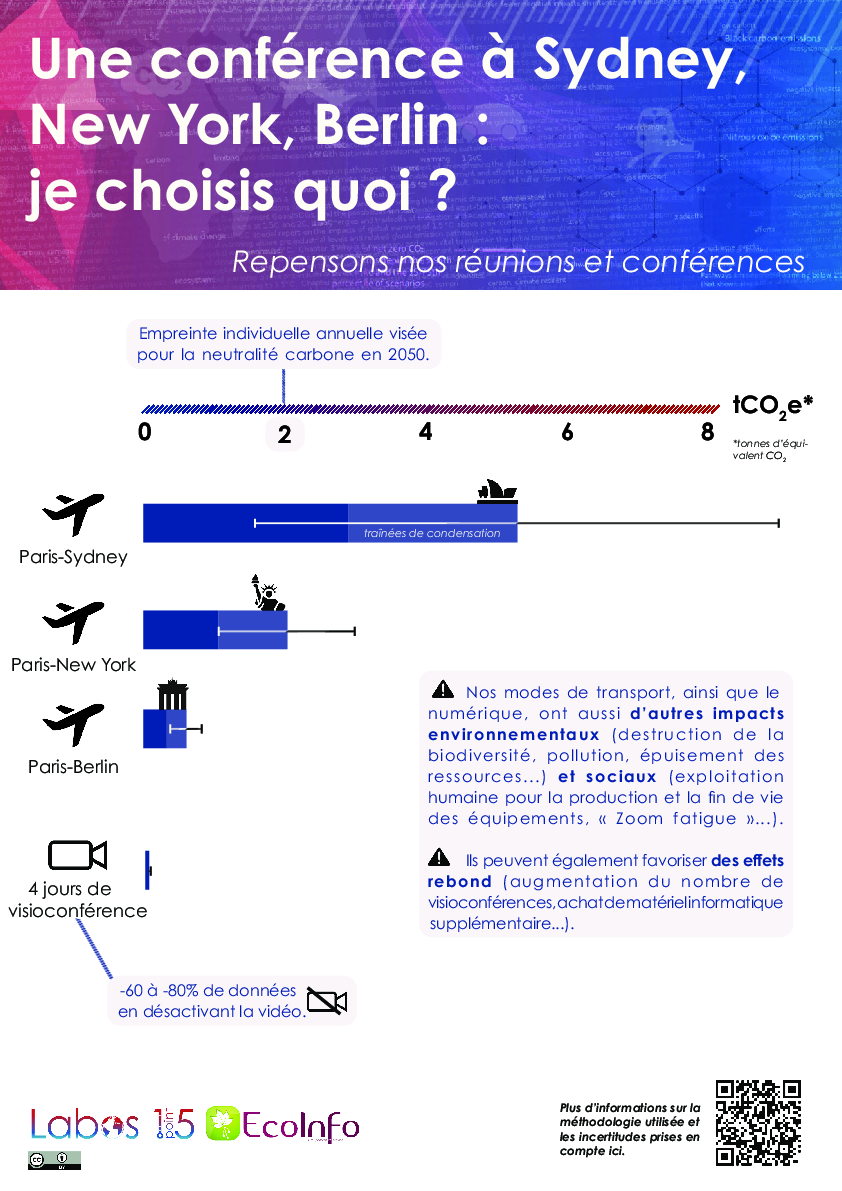
\includegraphics[width=0.5\textwidth]{images/sydney_v7_fr.png}
    \caption{Empreinte carbone s'une conférence à Sydney}
    \label{fig:sydney}
\end{figure}

\newpage

\begin{figure}[H]
    \centering
    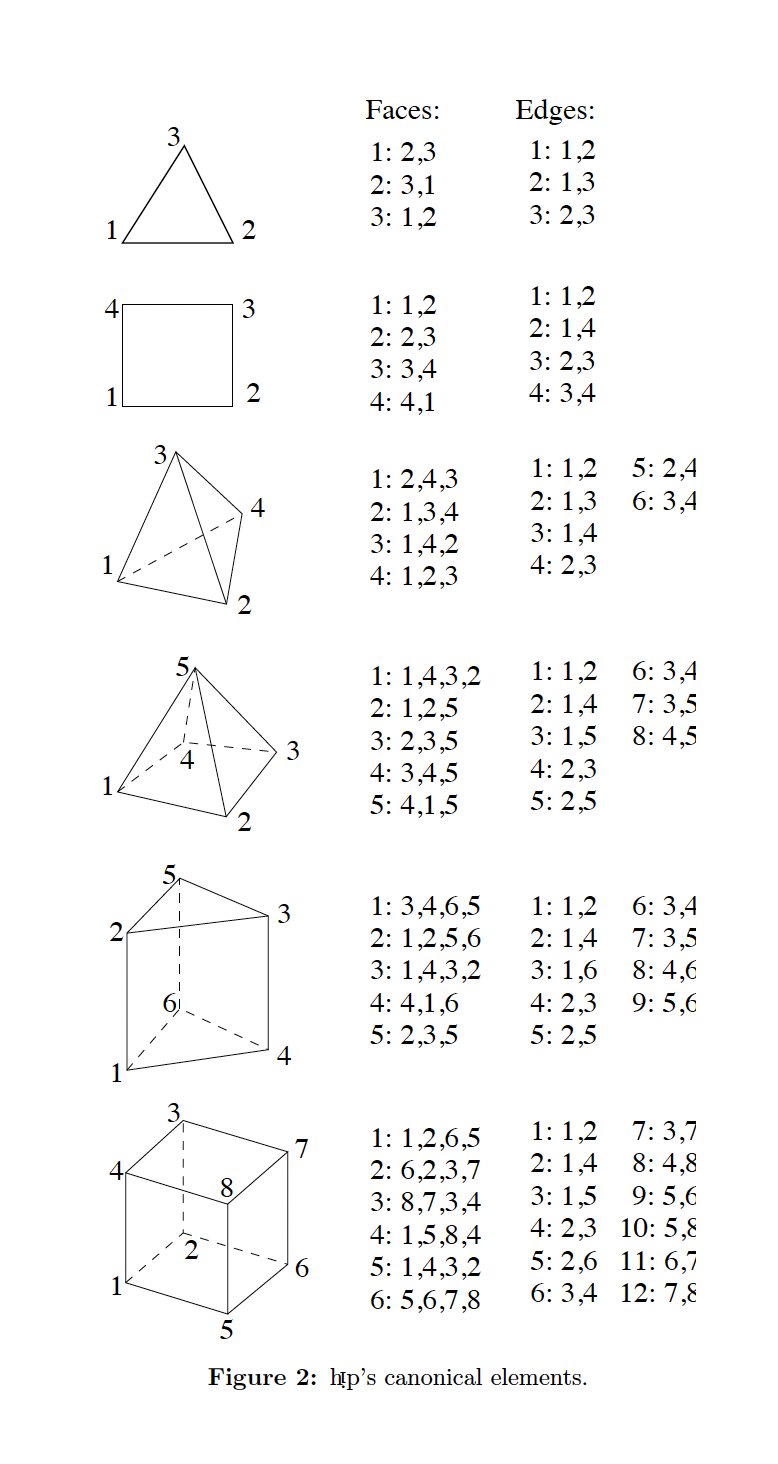
\includegraphics[width=0.39\textwidth]{images/Connectivite_hip.png}
    \caption{Connectivité dans hip}
    \label{fig:ordre_connect}
\end{figure}


\nocite{*}
\printbibliography
\addcontentsline{toc}{chapter}{Bibliographie}

\end{document}
